% Data generation
\section{Data generation}\label{sec:data}

\subsection{Cases and sampling}
We generate one single-transistor dataset per device and state. The case fixes $V_G$ and $V_B$;
all other inputs are drawn per row (Table~\ref{tab:ranges}), with $V_{DD}$ first because the
$V_D$, $V_S$ ranges depend on it. NMOS and PMOS process parameters are drawn separately around
the nominal values parsed from the card.

\begin{table}[H]
  \centering
  \small
  \caption{The four cases and the sampled inputs (base distribution, before oversampling).}
  \label{tab:ranges}
  \begin{tabular}{@{}lll@{}}
    \toprule
    \multicolumn{3}{@{}l}{\textbf{Fixed per case}} \\
    \multicolumn{3}{@{}l}{\texttt{nmos\_on}: $V_G=V_{DD}$, $V_B=0$; \quad
      \texttt{nmos\_off}: $V_G=0$, $V_B=0$;} \\
    \multicolumn{3}{@{}l}{\texttt{pmos\_on}: $V_G=0$, $V_B=V_{DD}$; \quad
      \texttt{pmos\_off}: $V_G=V_B=V_{DD}$} \\
    \midrule
    \textbf{Sampled} & \textbf{Range} & \\
    $V_{DD}$ & \VDDmin{} to \VDDmax & uniform \\
    $V_D$, $V_S$ & $0$ to $V_{DD}$ of the row & uniform \\
    $W$ & \WMultMin{} to \WMultMax{} $\times L_{\min}$ & uniform \\
    $T$ & \TempMin{} to \TempMax & uniform \\
    \texttt{vth0}, \texttt{toxe}, \texttt{ndep}, \texttt{u0}, \texttt{xj} & nominal $\pm$\ProcessTol &
      uniform, NMOS and PMOS separately \\
    \bottomrule
  \end{tabular}
\end{table}

\subsection{Oversampling the operating points gates actually use}\label{sec:oversampling}
Our first models were trained on uniform $V_D$, $V_S$ and failed badly inside gates
(Section~\ref{sec:history}): uniform sampling almost never produces the bias points a transistor
sees in a static gate, and a regression model is weakest where it has few neighbours. We
therefore replace part of the uniform draws with five rules, each tied to a specific in-gate
operating point. All draws stay inside the ranges of Table~\ref{tab:ranges}, and overridden
voltages are rounded to the printed precision, so stored inputs equal simulated ones.
\begin{itemize}
  \item \textbf{Low $|V_{DS}|$ (ON).} An ON transistor in a static gate connects two nodes at
        almost the same voltage. In \LowVdsFrac{} of ON rows, $|V_{DS}|$ is log-uniform in
        [\LowVdsMin, \LowVdsMax] with random sign.
  \item \textbf{Source pinning (OFF).} An OFF transistor has its source on its own rail, or a
        small offset away inside a stack. In \SourcePinFrac{} of OFF rows, $V_S$ = rail + an offset
        log-uniform in [\PinMin, \PinMax].
  \item \textbf{Drain pinning (OFF).} The OFF transistor that sets a gate's leakage also has its
        drain on the opposite rail. An independent \DrainPinFrac{} of OFF rows get $V_D$ = opposite
        rail minus an offset with the same law, so about \BothPinFrac{} sit at the full-$V_{DD}$
        OFF point.
  \item \textbf{Stack pinning (ON).} The upper NMOS of a stack (NAND2 \texttt{10}) is ON with its
        drain at $V_{DD}$ but its source on a floating internal node, a threshold below the
        supply; NOR2 \texttt{10} has the PMOS mirror. About \qty{15}{\percent} of ON rows get the
        drain on the far rail and the source \numrange{0.03}{0.5}\,$V_{DD}$ away from it.
  \item \textbf{Boundary rows (all).} In \BoundaryFrac{} of rows, each of \BoundaryInputs{} is,
        with probability \BoundaryPerInput, redrawn from the outer \BoundaryBand{} of its range,
        because tree models degrade at the box edges and the PVT corners reach them.
\end{itemize}

We want to be explicit about how these rules were found: the gate-level error analysis told us
\emph{which} operating points were under-sampled. To avoid fitting the sampling to our evaluation
data, every added range is deliberately wider than what the gates show, all model and
hyperparameter choices are made on transistor validation data only, and we repeated the gate
evaluation on fresh corners that were never inspected (Section~\ref{sec:fresh}).

\subsection{Dataset size, split and netlists}
Each case has \RowsPerCase{} rows instead of the proposed \num{10000}. A learning curve (refits on
nested subsets of the training split, scored on fixed validation rows) showed the error still
falling clearly at \num{7000} training rows: the \texttt{nmos\_off} $I_D$ median error drops from
\LCMedian{nmos_off}{id}{7000} at \num{7000} rows to \LCMedian{nmos_off}{id}{21000} at
\LCMaxSize{}, and the \texttt{nmos\_on} $I_G$ error from \LCMedian{nmos_on}{ig}{7000} to
\LCMedian{nmos_on}{ig}{21000} (Figure~\ref{fig:lc}). The curve falls more slowly beyond \num{14000} rows
but has not levelled off, so \RowsPerCase{} is a reasonable trade-off against SPICE and training cost.

Each dataset is split \SplitScheme{} (seed \SeedSplit) into \NTrain{} training, \NVal{}
validation and \NTest{} test rows; split indices are saved. Every row is one ngspice deck with
its own rewritten \texttt{.model} block and a separate DC source per terminal; currents are stored
positive \emph{into} the device ($I_D = -\texttt{i(vd)}$). Example decks are in
Appendix~\ref{sec:appnetlists}.

\begin{figure}[H]
  \centering
  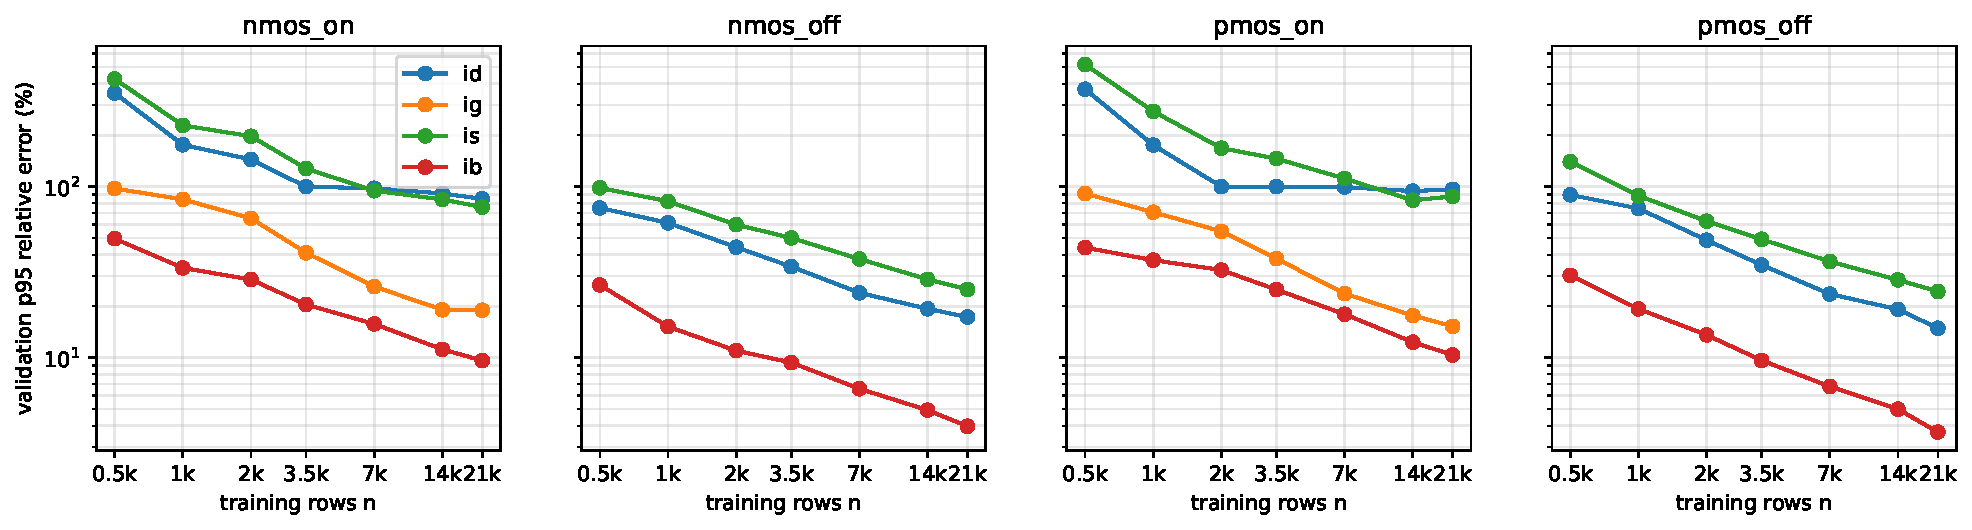
\includegraphics[width=0.85\linewidth]{learning_curve.pdf}
  \caption{Learning curve: validation p95 error of the chosen model recipe against training rows
  (log--log). Every curve still falls at \num{7000} rows. ON $I_D$/$I_S$ stay high for a different
  reason: their p95 is set by rows where the channel current crosses zero
  (Section~\ref{sec:errtrans}).}
  \label{fig:lc}
\end{figure}

\subsection{Data check}
\paragraph{Kirchhoff's law.}
The four terminal currents must sum to zero (Table~\ref{tab:kirchhoff}). For NMOS the relative
residual is at solver level (median \KirchhoffMedianRelNmosOn{} ON, \KirchhoffMedianRelNmosOff{}
OFF). For PMOS the absolute residual stays near $10^{-16}$\,A (p95 \KirchhoffPninetyfiveAbsPmosOn{}
ON, \KirchhoffPninetyfiveAbsPmosOff{} OFF), which we attribute to rounding in the body-resistance
network of \texttt{rbodymod=1}; it shows up in relative terms (up to \KirchhoffWorstRel) only
where all four currents are tiny. No row violates KCL beyond this floor, which also confirms our
sign convention.

\begin{table}[H]
  \centering
  \small
  \caption{Kirchhoff check (D3): residual $|I_D+I_G+I_S+I_B|$ over all \RowsPerCase{} rows per case.}
  \label{tab:kirchhoff}
  \fittable{% Generated by report/make_numbers.py from results/tables/kirchhoff.csv. Do not edit.
\begin{tabular}{lrrrrrr}
\toprule
 & \multicolumn{3}{c}{$|I_D+I_G+I_S+I_B|$ (A)} & \multicolumn{3}{c}{relative to $\max|I|$} \\
\cmidrule(lr){2-4}\cmidrule(lr){5-7}
Case & median & p95 & max & median & p95 & max \\
\midrule
\texttt{nmos\_on} & \num{4.0e-20} & \num{4.6e-16} & \num{9.7e-15} & \num{1.1e-11} & \num{1.4e-10} & \num{3.7e-08} \\
\texttt{nmos\_off} & \num{1.1e-24} & \num{4.8e-22} & \num{9.9e-21} & \num{1.2e-11} & \num{5.9e-11} & \num{1.1e-10} \\
\texttt{pmos\_on} & \num{3.3e-17} & \num{3.0e-16} & \num{9.1e-15} & \num{8.0e-09} & \num{3.1e-03} & \num{1.3e-02} \\
\texttt{pmos\_off} & \num{2.6e-17} & \num{7.2e-17} & \num{1.7e-16} & \num{1.5e-04} & \num{4.7e-03} & \num{8.5e-02} \\
\bottomrule
\end{tabular}
}
\end{table}

\paragraph{Trends.}
Figure~\ref{fig:trends} confirms the expected physics: the OFF current rises exponentially with
temperature and falls exponentially with $|V_{th0}|$ (subthreshold conduction), and the gate
current falls exponentially with \texttt{toxe} (tunnelling), with the ON cases many decades above
the OFF cases, where only the gate--drain overlap tunnels. The flat floor near $10^{-14}$\,A in the
OFF current is BSIM4's default junction current, since the decks give no junction areas.

\begin{figure}[H]
  \centering
  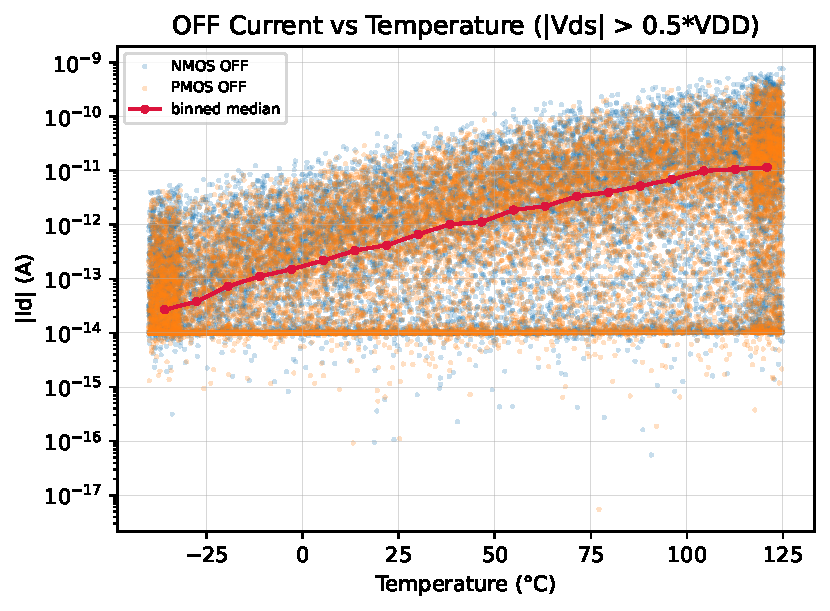
\includegraphics[width=0.32\linewidth]{trend_ioff_vs_temp.pdf}\hfill
  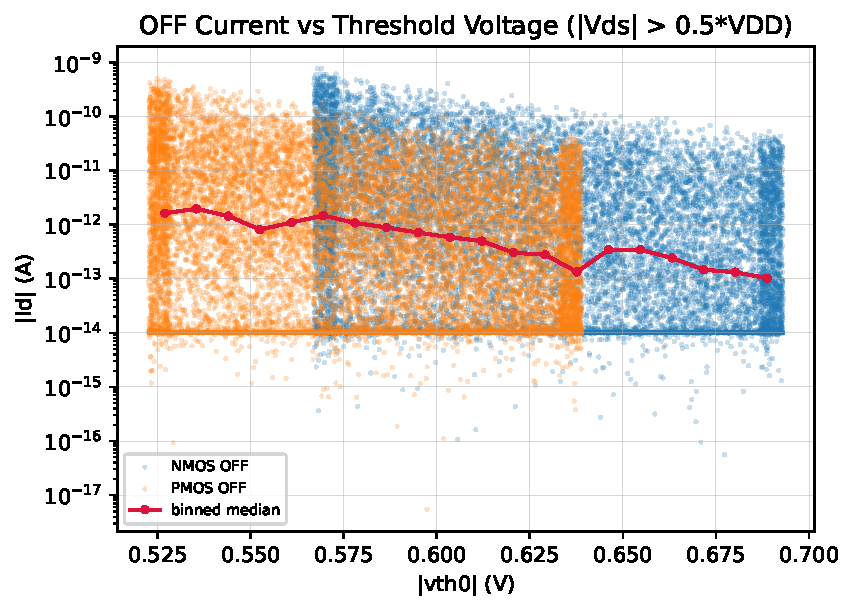
\includegraphics[width=0.32\linewidth]{trend_ioff_vs_vth0.pdf}\hfill
  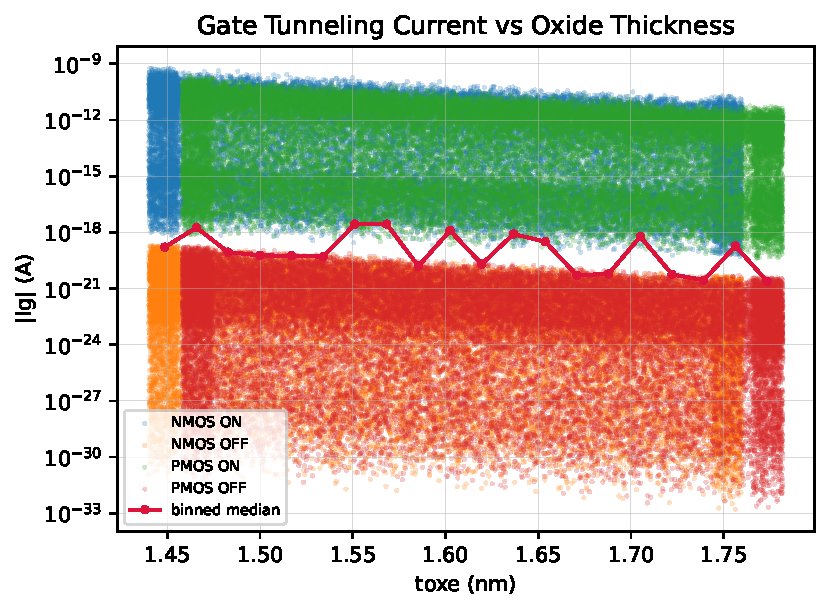
\includegraphics[width=0.32\linewidth]{trend_ig_vs_toxe.pdf}
  \caption{Data-check trends (D3): OFF drain current vs temperature (left) and vs $|V_{th0}|$
  (centre); gate current vs \texttt{toxe} for all cases (right). Dense strips at the range edges
  are the boundary rows.}
  \label{fig:trends}
\end{figure}
